\documentclass[10pt,twocolumn,letterpaper]{article}

\usepackage{cvpr}
\usepackage{times}
\usepackage{epsfig}
\usepackage{graphicx}
\usepackage{subcaption}
\usepackage{amsmath}
\usepackage{amssymb}

% Include other packages here, before hyperref.

% If you comment hyperref and then uncomment it, you should delete
% egpaper.aux before re-running latex.  (Or just hit 'q' on the first latex
% run, let it finish, and you should be clear).
\usepackage[pagebackref=true,breaklinks=true,letterpaper=true,colorlinks,bookmarks=false]{hyperref}

\cvprfinalcopy % *** Uncomment this line for the final submission

\def\cvprPaperID{****} % *** Enter the CVPR Paper ID here
\def\httilde{\mbox{\tt\raisebox{-.5ex}{\symbol{126}}}}

% Pages are numbered in submission mode, and unnumbered in camera-ready
\ifcvprfinal\pagestyle{empty}\fi
\begin{document}

%%%%%%%%% TITLE
\title{Image Colorization via Conditional Generative Adversarial Network}

\author{Luan Tran\\
Michigan State University\\
{\tt\small tranluan@msu.edu}
% For a paper whose authors are all at the same institution,
% omit the following lines up until the closing ``}''.
% Additional authors and addresses can be added with ``\and'',
% just like the second author.
% To save space, use either the email address or home page, not both
\and
Saif M. Imran\\
Michigan State University\\
{\tt\small imransai@msu.edu}
}

\maketitle
%\thispagestyle{empty}

%%%%%%%%% ABSTRACT
\begin{abstract}
We aim to color gray-scale images automatically, without direct human assistance.
This automatic colorization is an underconstrained problem 
since there is usually no one-to-one correspondence between color and local texture.
In this work, we will try to apply recent advances in generative models which is Generative Adversarial Network~\cite{goodfellow2014generative} (GAN) to a conditional setting. Instead of generate realistic samples from random noise as conventional GAN, we will generate realistic samples (color image) from both input gray-scale image and noise.
\end{abstract}

%%%%%%%%% BODY TEXT
\section{Introduction}

Automated colorization of gray-scale images has been subject to much research within the computer vision and machine learning communities. Beyond simply being fascinating from an aesthetics and artificial intelligence perspective, such capability has broad practical applications ranging from video restoration to image enhancement for
improved interpretability. 

At first glance, hallucinating image colors seems daunting, since so much of the information (two out of the
three dimensions) has been lost. However, the semantics of the scene and its surface texture provide ample cues for many regions in each image. For this work, our goal is not necessarily to recover the actual ground truth color, but rather to produce a plausible colorization that could potentially fool a human observer. Therefore, our task becomes much more achievable: to model enough of the statistical dependencies between the semantics and thevtextures of grayscale images and their color versions in order to produce visually compelling results.

%------------------------------------------------------------------------
\section{Proposed approach}


\begin{figure} [t!]
    \centering
    \begin{subfigure}[b]{0.48\textwidth}        
        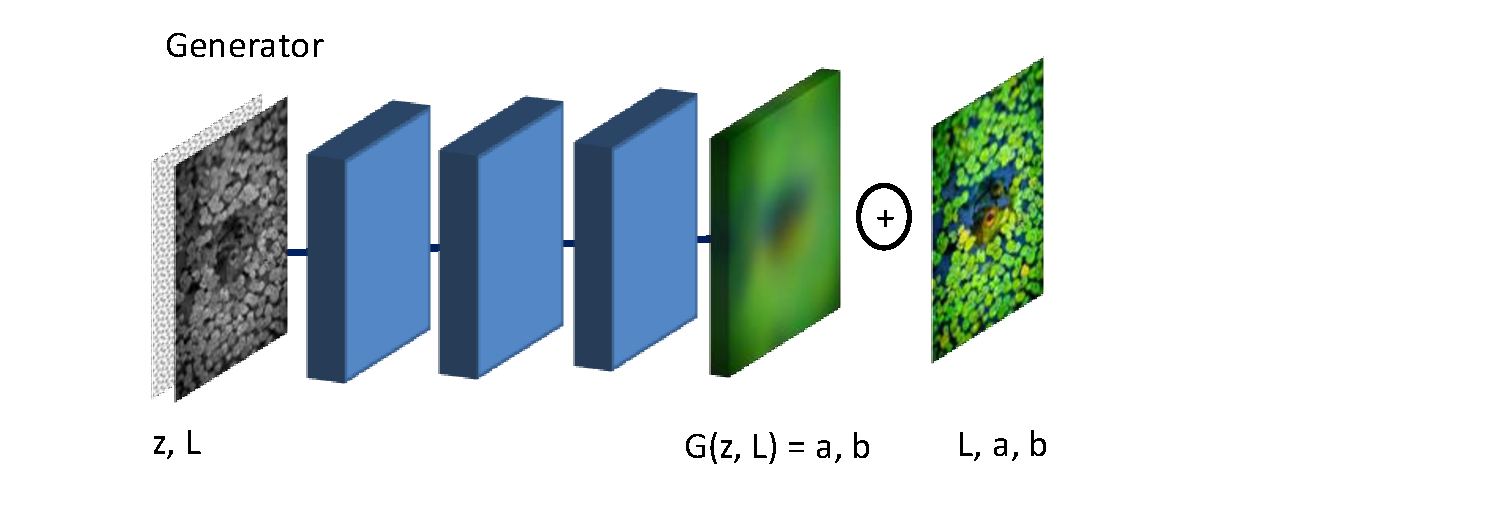
\includegraphics[trim=30 20 150 0, clip,width=\textwidth]{img/Generator.pdf}
    \end{subfigure}
    \begin{subfigure}[b]{0.48\textwidth}
        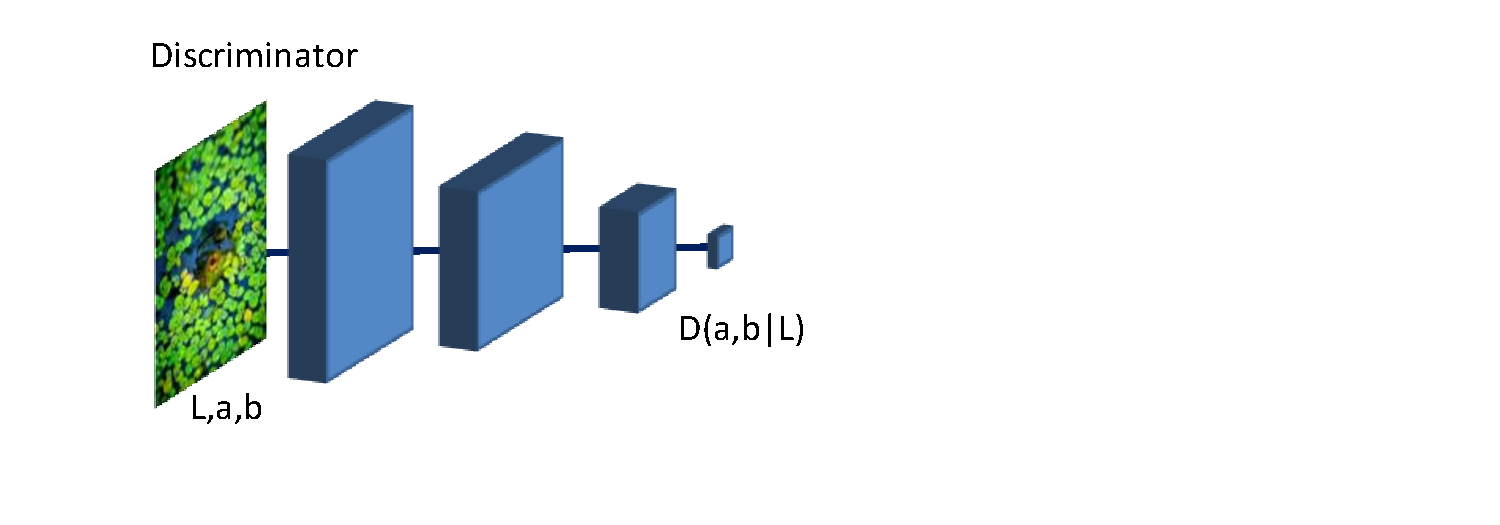
\includegraphics[trim=30 20 150 0, clip,width=\textwidth]{img/Discriminator.pdf}
    \end{subfigure}
    \vspace{-0.16in}
    \caption{\small Network architecture.}
    \vspace{-0.2in}
   \label{fig:dataPartition}
\end{figure}

Each color image can be presented in Lab space. Any gray-scale input image can be treat as lightness component (L) of the final color out. Thus, we only need to estimate a, b component. The system consist of two network: generator ($G$) and discriminator ($D$). The generator take the gray-scale image ($L$) and random noise ($z$) as inputs and try to produce $a, b$ component of the image. Meanwhile D take all three components of images as inputs and try to distinguish between samples from the training data and generated samples. In other word, $D$ will produce one single value $D(a,b|L)$ that is probability $a, b$ is the true color component correspond to $L$. Both network $G, D$ will be train to optimize this function:
\begin{eqnarray*}
 \min_{G} \max_{D} V(G,D) = &&E_{a, b \sim p_{data}(a,b | L)} [\log(D(a,b|L))] \\ 
                          + &&E_{z \sim p(z), L \sim p_{data}(L) } [\log(1-D(G(z,L)))]
\end{eqnarray*}


In order to deal with any input size, $G$ will be a fully convolutional network as inspired by~\cite{long2015fully}. All convolution filter has size $3 \times 3$ as it has been shown to be effective in lasted CNN.

\section{Experiments & Evaluation}
Our networks will be train and test on ImageNet dataset. To simplify the setup for D, all the training samples will have fixed size of $64\times 64$. In the test state, sample images with any size can be used since it only go though the generator $G$.

Because of the nature of the task, it's difficult to come up with a quantitative metrics to evaluate the performance. We're going to create a UI for people to decide which is more realistic between generated and ground truth images. This can give a sense to what extend our generated images can fool human.  



{\small
\bibliographystyle{ieee}
\bibliography{egbib}
}

\end{document}
